%% LyX 2.3.6 created this file.  For more info, see http://www.lyx.org/.
%% Do not edit unless you really know what you are doing.
\documentclass[10pt]{article}
\usepackage{helvet}
\renewcommand{\familydefault}{\sfdefault}
\usepackage[T1]{fontenc}
\usepackage[utf8]{inputenc}
\usepackage[a4paper]{geometry}
\geometry{verbose,tmargin=2cm,bmargin=4cm,lmargin=2cm,rmargin=2cm}
\usepackage{fancyhdr}
\pagestyle{fancy}
\setlength{\parskip}{6pt}
\setlength{\parindent}{0pt}
\usepackage{tcolorbox}
\usepackage{amsmath}
\usepackage{amsthm}
\usepackage{amssymb}
\usepackage{todonotes}
\usepackage{graphicx}
\usepackage[backend=bibtex,maxbibnames=99]{biblatex}
\addbibresource{main.bib}

\makeatletter

%%%%%%%%%%%%%%%%%%%%%%%%%%%%%% LyX specific LaTeX commands.
%% A simple dot to overcome graphicx limitations
\newcommand{\lyxdot}{.}


%%%%%%%%%%%%%%%%%%%%%%%%%%%%%% User specified LaTeX commands.
\usepackage{tcolorbox}
\usepackage{amsthm}
\usepackage{lastpage}
\usepackage{fancyhdr}
\usepackage{accents}
\usepackage{titlesec}
\usepackage{marginnote}
\usepackage{titlesec}
\titleformat{\section}[block]{\normalfont\bfseries}{}{0em}{}


\usepackage{enumitem}
\usepackage{comment}
\setlist{nolistsep}

\usepackage{tcolorbox}
\definecolor{light-blue}{cmyk}{0.24, 0.12, 0.0, 0.04, 1.00}
\titlespacing\section{0pt}{0pt}{0pt}
\titlespacing\subsection{0pt}{0pt}{0pt}
\titlespacing\subsubsection{0pt}{0pt}{0pt}

\setlength{\headheight}{40pt}

\makeatother

\begin{document}
\lhead{Neimhin Robinson Gunning} \rhead{CS7CS4 Final Assignment}

\section{DublinBike Usage}
Here we investigate the impact of the coronavirus pandemic on
DublinBike usage, by comparing forecasts based on pre-pandemic data
with the recorded usage during and after the pandemic period.

The first unilateral government guidelines in Ireland regarding
mitigation of viral spread were issued and came into affect on
the 12th of March 2020 \cite{leahy2020coronavirus}. For the purposes of this investigation
we regard this date as the start of the pandemic era. This is
admittedly somewhat arbitrary; cases of Covid-19 were recorded earlier
in Feb 2020.
We consider 28th February 2022 as the end of the pandemic in Ireland
because on this date almost all public health restrictions were lifted \cite{molony2022almost}.
Again this is somewhat arbitrary.

% Reportedly:
% ``Data released by Dublin City Council to this website shows that usage
% last year was still around 1.8 million trips down from pre-pandemic levels
% — with 2,001,810 trips by users in 2022 compared to 3,816,652 in 2019.'' \cite{ginty2023dublinbikes}.

\subsection{Engineering a ``usage'' feature}
The dublin bike data set used for this analysis consists
of snapshots of station occupancy, for the most part at five-minute intervals,
but a large portion of the data set instead uses thirty minute intervals.
Since the purpose of this analysis is to compare different eras, we have decided
to thin the entire data set, using only snapshots at time multiples of 30 minutes,
such that the sampling interval is consistent for each subset of the data.
Admittedly we are leaving data on the table that could be used
to improve confidence in our analyses, and with more time it would have
been interesting to develop a solution to leveraging the more 
dense data while keeping the comparison fair.

% First we thin all of the data, keeping only snapshots taken at intervals of 30 minutes.
% We do this because a significant portion of the data set uses only 30 minute, rather than 5 minute, snapshots.
% It is only the pandemic and post-pandemic era data that have this sampling style.
% Since the purpose of the analysis is to compare the different eras,
% we thin the data such that the sampling style is consistent throughout the data set.

The data set does not include direct information about individual interactions
with the bike stations, such as renting a bike or returning a bike to the station.
Because of this it is not possible to determine from the
data set the exact number of journeys in a given time period,
which would be an ideal usage metric.

We have considered three approaches to approximating bike usage.

The first approach is to estimate the total number of bikes in operation.
At each time interval we can count up the total number of available bikes across all stations.
Considering each time point during one day, we can take the maximum number of available bikes,
which usually falls at some time in the early hours of the morning, between 1am and 5am.
The total number of bikes in the system apparently changes regularly. Once an estimate
for the total number of bikes has been established we can then estimate the total number of bikes
in use at a given time by subtracting the total 'available' bikes (bikes parked at a station) from the estimated total bikes in operation.

A second approach involves counting up how many times a bike station has been interacted with
over a given interval. We can detect an interaction by checking whether the last update to the
bike station occurred {\em after} the previous update, i.e. $\textsc{LAST UPDATED} > \text{TIME} - 30\text{minutes}$.
Additionally, we can use the difference between the current time and the last update to get some information
about the frequency of interactions. If the last update happened very recently then there is a higher likelihood of the
frequency of interactions being high, and if the last update happened long ago this is evidence that the frequency of interactions
is low.
There is an issue with this approach due to an apparent bug in how the data set was created.
There are cases where the snapshot seemingly misreports \textsc{last updated}. In the below snippet
the second row shows that there was an update at 22:13, but the snapshot for 22:15 indicates the last update was at 22:08.

{\centering
\begin{tabular}{r r r}
     STATION ID &                TIME &        LAST UPDATED \\
              2 & 2018-08-01 22:15:03 & 2018-08-01 22:08:30 \\
              2 & 2018-08-01 22:20:01 & 2018-08-01 22:13:50 \\
%              2 2018-08-01 22:25:01 2018-08-01 22:20:24
\end{tabular}
}

This is a contradiction.
It is possible to detect and clean these errors automatically, but the error raises suspicions about the accuracy of the data set.

The third approach we have considered involves looking at the change in station occupancy between intervals.
We can look at the difference in bike occupancy at the
beginning and end of a 30 minute interval to establish
a {\em lower-bound} on the number of interactions with
the station, but it is possible for there to have been
more interactions (returns or borrowings) than this difference.
For instance, it may be that a bike station has 10 bikes at time $t$
and 10 bikes at time $t+30\text{m}$, but that in fact 5 bikes were
borrowed {\em and} 5 bikes were deposited.

We can detect such cases, because the data set also includes a
\textsc{last updated} field. If the occupancy is not changed, but 
the time of last update is between the start and end of the interval,
then we know that there were at least 2 interactions with the bike station.
In such cases there can only have been an even number of interactions, ${2,4,6,\ldots}$, and we
could go further to assume a geometric distribution over these possibilities.

A problem we see with this approach is that the difference in occupancy is limited to
the number of bike terminals at the station.
Let's say a station has 20 terminals.
If there is a time when a station is experiencing 100 times as much usage as normal,
this will not be reflected in that stations change in occupancy, because the change is capped to 20.

However, instead of looking at the change in occupancy of just a single station,
we can compute the global bike station occupancy at a given time, and then compute
the difference in global occupancy between intervals. This number will be sometimes
negative and sometimes positive, but both positive and negative values imply usage.
The question remains whether a positive difference (more available bikes) in occupancy or a negative
difference (fewer available bikes) indicates higher usage.
For this analysis we treat positive and negative
differences the same, and so take the absolute value of the global occupancy difference as
a proxy measure for usage at each 30 minute interval.
This is the pseudo-usage metric we use for our analysis.

% We compute the \textsc{has changed} column by $$\textsc{has changed}_i = 
% \begin{cases} 
% 1 & \text{if } \textsc{LAST UPDATED}_i > \textsc{TIME}_{i - 1} \\
% 0 & \text{otherwise}
% \end{cases}
% $$ and then $$\textsc{missed change}_i = \textsc{has changed}_i \land (\textsc{diff}_i = 0)$$

% Considering occupancy data spanning 1st Jan 2020 to 1st Apr 2020, \textsc{missed change} is true
% about for about 37\% ($828673/2228278$) of the intervals.
% We must also remember that there are cases where \textsc{available bikes} has changed, but the difference in occupancy does not reflect the true number
% of interactions. There is no way to detect these cases.

% But is it possible to get more information about this
% distribution from the data?
% Yes, if we can estimate the rate of bike removals.

% Something we can estimate without caveats is the distribution of time since the last update.


% \subsubsection{Usage over time}
% % LOWER BOUND TAKE OUTS
% % note that the 2018 and 2023 years are incomplete
% % YEAR  LOWER BOUND JOURNEYS
% % 2018             2603824.0
% % 2019             5721975.0
% % 2020             5194359.0
% % 2021             5308306.0
% % 2022             1074247.0
% % 2023             1062018.0

% % YEAR           NUM SAMPLES
% % 2018               4937925
% % 2019              10691784
% % 2020              10896643
% % 2021              11157202
% % 2022               1982257
% % 2023               1972740

% % YEAR   AVAILABLE BIKES DIFF RELU
% % 2018                     1094039
% % 2019                     2334214
% % 2020                     1358085
% % 2021                     1357736
% % 2022                     9564400
% % 2023                     9860396

% % irishcycle.com report
% % YEAR          NUM JOURNEYS
% % 
% % 2019               3816652
% %
% %
% % 2022 	             2001810

% \subsubsection{A `usage' feature based on \textsc{last updated}}
% Because of all the severe caveats with the difference based `usage' features
% we seek an alternative based on the \textsc{last updated} column.
% First, we assume variable, the arrival rate, which changes over time.
% The arrival rate is the expected number of uses of a bike station per minute.
% We can estimate the arrival based on the \textsc{last updated} variable.

% For each snapshot the station's state we can calculate the amount of time since the last update, $\Delta t$.
% Absent of other contextual evidence, the inverse of this is the best estimate of the arrival rate, $\lambda_{[\text{user/minute}]} = \frac{1}{\Delta t}$.
% Since samples are taken every 5 minutes, we can then multiply the arrival rate by 5 minutes 
% to estimate the number of interactions with the bike station,
% $\hat{\text{\#interactions}} = 5 \times \lambda$.
% This calculation yields the unfortunate result where time intervals that are
% known to have no interactions will have a small non-zero number of estimated interactions.

% We can further adjust the estimation of the arrival rate by aggregating across more samples, e.g.
% for an hour interval, take the average of \textsc{last updated}, and use $\hat{\text{\#interactions}} = 60 \times \lambda$.
% Or, for a particular time of day, aggregate across multiple days, etc.

% There is a problem with this approach due to an apparent bug in how the data set was created.
% There are cases where the snapshot seemingly misreports \textsc{last updated}. In the below snippet from
% the second row shows that there was an update at 22:13, but the snapshot for 22:15 indicates the last update was at 22:08.
% This is a contradiction.
% %      STATION ID                TIME        LAST UPDATED
% %               2 2018-08-01 22:15:03 2018-08-01 22:08:30
% %               2 2018-08-01 22:20:01 2018-08-01 22:13:50
% %               2 2018-08-01 22:25:01 2018-08-01 22:20:24

% We have intentionally avoided the use of lagged features, e.g. to predict the usage at time $t$, aggregate data from times $t-n,t-2n,\ldots$, for the reason
% that such features would themselves have to be estimated when making predictions outside the pre-pandemic era.
% This would result in wilder and less interpretable predictions.

In summary, there is no way to accurately derive a semantically precise usage metric from the
data set, such as the number of journeys, or the amount of rental time.
We must settle for a proxy usage metric. We define our pseudo-usage metric based the global
change in the number of available bikes.

We group samples by time interval and sum \text{AVAILABLE BIKES} for all stations, to get the global number
of available bikes $g_t$ at each point in time.
Our usage statistic $u_{\text{30m}}$ is then the absolute value of the difference between $g_t$ at subsequent intervals: $u_{\text{30m}^t}=|g_t-g_{t-\text{30m}}|$.
For analysis, we also use an aggregated version of this metric, summing $g_t$ over different lengths of time, e.g. one month,
$$ u_\text{M}=\sum_{t\in M}g_t $$.

\subsection{Forecasting Usage}
To forecast (counterfactually) DublinBike usage in the pandemic and post-pandemic eras we isolate the
pre-pandemic DublinBike data for model development and evaluation.

We notice that the distributions for working days and non-working days are obviously different, and thus
we use a baseline predictor based on two subsets of the data, working days and non-working days.
This `split baseline' uses the mean pseudo-usage of both subsets for predictions:
$$\hat{u}_i = 
\begin{cases} 
E[u|\text{workday}] & \text{if workday} \\
E[u|\lnot\text{workday}] & \text{if not workday}
\end{cases}
$$

The input features for forecasting are:
\begin{itemize}
    \item \textsc{timestamp}: The Unix epoch time of the sample rounded to the nearest thirty minutes.
    \item \textsc{workday}: Whether or not the sample was taken on a workday. Set to 0 for non-workdays, including weekends, bank holidays, and national holidays, 1 for workdays.
    \item \textsc{interval}: A one-hot encoding of the time of day. With sample frequency of 30 minutes there are 48 intervals, and thus this one-hot vector has length 48.
\end{itemize}

We use a pair of Lasso linear regression models, one trained on the `workday' subset, and the other
trained on the `non-workday' subset. We call this the `dual lasso' predictor.
We found that a single lasso model performed much worse than the `split baseline'.

Each lasso model has $48+1+1=50$ trainable parameters we call $\theta$.
The input features are arranged in a vector of length 51, with one dummy feature that is always 1: $$x=[1,\text{timestamp},\ldots\text{interval one-hot}]$$
The model for prediction is then $\hat{y}(x) = \theta^{\intercal}x$.
The model for prediction of the dual lasso model is therefore $$
\begin{cases}
    \hat{y}_{\text{workday}}(x_t)     & \text{if } t \in \text{workdays} \\
    \hat{y}_{\text{non-workday}}(x_t) & \text{if } t\notin \text{workdays}
\end{cases}    
$$.

This model inherently enforces a prediction of approximately linear growth rate of usage,
but accounts for the fact that there are
different numbers of holidays for different time intervals.
The pre-pandemic era data spans less than 2 years which is
arguably not enough data to detect non-linear growth rate year-on-year,
so we decided to choose a model which inherently can not predict exponential or geometric growth.

The hyperparameter $\alpha$ is selected independently for each of the `dual lasso' submodels.
5-fold cross-validation, without shuffling of data, is used. The reason not to shuffle the data
is that we are trying to forecast usage well outside the domain of the training data.
By not shuffling we ensure that a larger portion of the test data is further outside the time-domain
seen in the training data, meaning we are evaluating the model's ability to generalize to new time-intervals.
The 5 splits used for tuning of Alpha via cross-validation, as well as the cross-validation results are presented in Figure \ref{fig:hyperparameter}.

\begin{figure}
    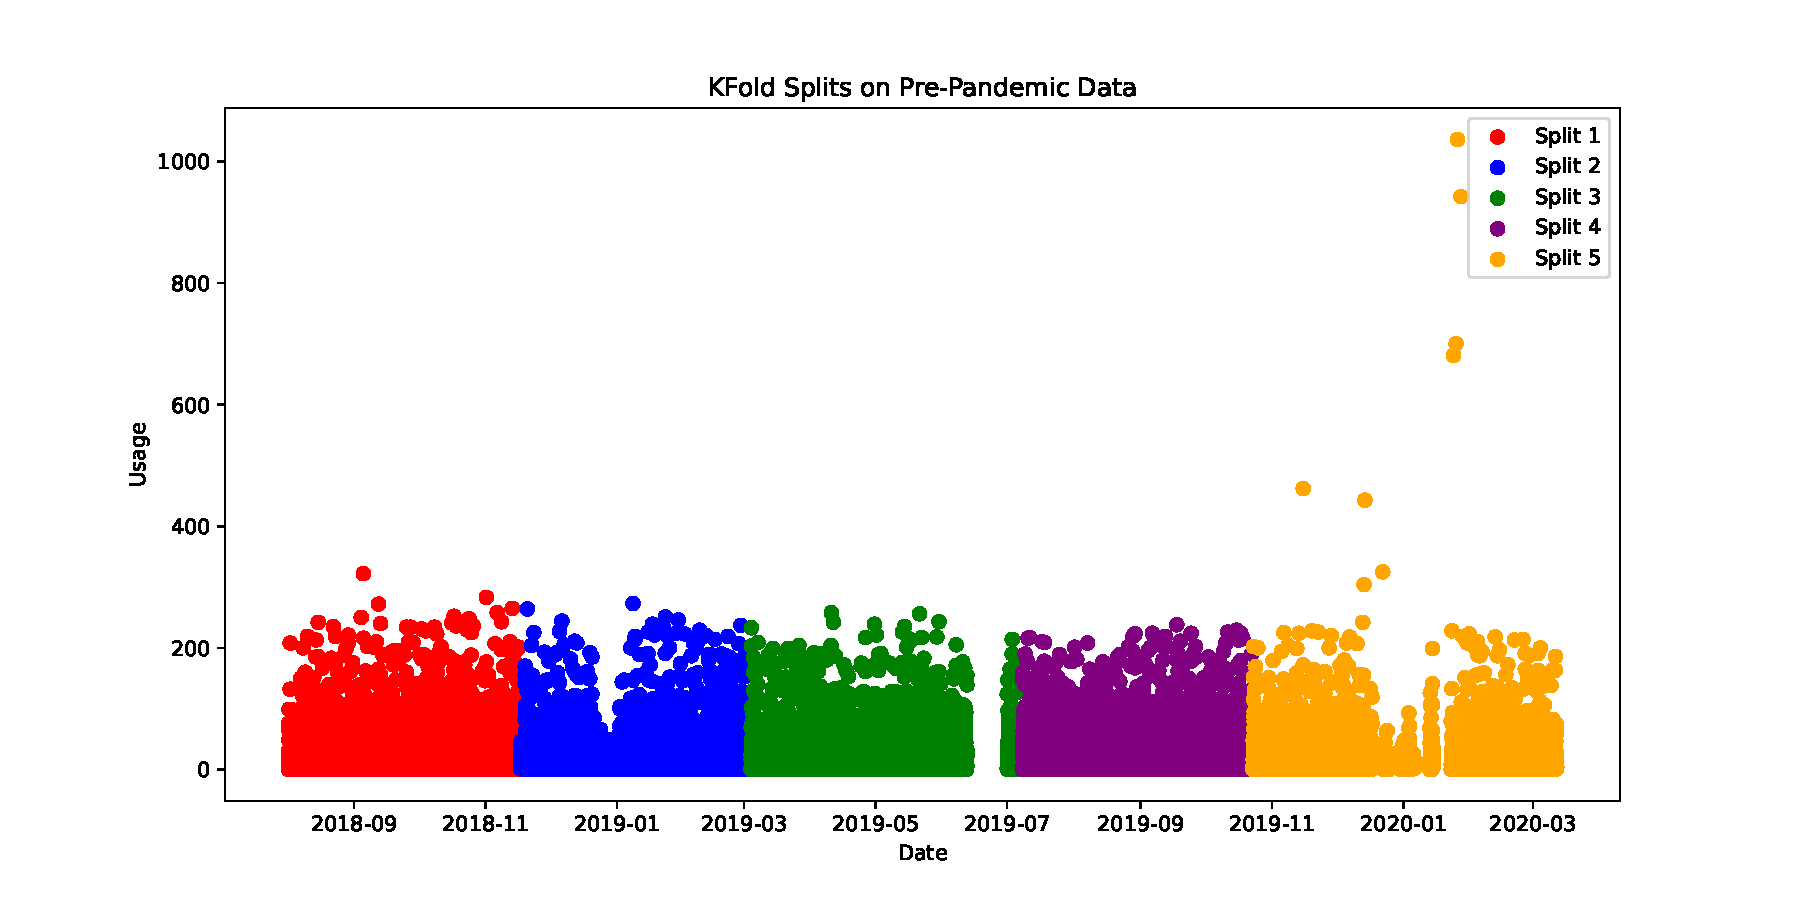
\includegraphics[width=\textwidth]{merged-all-30min.csv.d/pre-pandemic-cross-val-split.pdf}
    \includegraphics[width=\textwidth]{merged-all-30min.csv.d/dual\_lasso\_hyperparameter\_tuning.pdf}
    \caption{Above: The 5 splits used in cross-validation. Below: The mean and standard deviations of the MSEs for the two submodels. Here the
    MSE score is calculated on just the respective subsets (workday, non-workday). To balance performance and regularization we set C to $10^2$ for both models.}
    \label{fig:hyperparameter}
\end{figure}

% best workday alpha: 0.01743328822199987 C: 57.361525104486816
% best non workday alpha: 0.0016102620275609393 C: 621.0169418915616

% Comparing dual lasso model to split baseline.
% workday mean 20.49938841540404
% non workday mean 9.810360736411969
% dual model mse: 977.0018326489687
% baseline model mse: 1166.640512328726
In Table \ref{tab:temporal-granularities-cross-val} we present cross-validated MSE scores of the `dual lasso' and `split baseline' predictors
after aggregating at various temporal granularities. The scores suggest that the dual lasso model has better performance at shorter granularities (30m, day), but
the baseline model makes better predictions for longer granularities (week, month).
% mse on time dual lasso  mse on time baseline  mse on day dual lasso  mse on day baseline  mse on week dual lasso  mse on week baseline  mse on month dual lasso  mse on month baseline
% count                5.000000              5.000000               5.000000             5.000000            5.000000e+00          5.000000e+00             5.000000e+00           5.000000e+00
% mean               790.413194           1213.577859           54638.558540         53851.589714            1.169966e+06          9.544779e+05             1.169966e+06           9.544779e+05
% std                312.696876            231.063726           25999.064370         27513.377553            6.990328e+05          5.127416e+05             6.990328e+05           5.127416e+05
% \begin{table}
% \begin{tabular}{r r}
%                & 30 minute  \\
%     baseline   & 1214 ± 231 \\
%     dual lasso & 790 ± 312  \\
% \end{tabular}
% \end{table}

\begin{table}[h]
    \centering
    \begin{tabular}{|l|c|c|}
    \hline
    Time Frame & Baseline (MSE mean ± std) & Dual Lasso (MSE mean ± std) \\
    \hline
    30 minute & 1214 ± 231 & 790 ± 313 \\
    Day       & 53852 ± 27513 & 54639 ± 25999 \\
    Week      & 954478 ± 512742 & 1169966 ± 699033 \\
    Month     & 8795224 ± 6288837 & 11750170 ± 8206649 \\
    \hline
    \end{tabular}
    \caption{Comparison of cross-validated MSE of `split baseline' and `dual lasso' predictions of pseudo-usage at various temporal granularities.
    The data used here is the pre-pandemic data only.}
    \label{tab:temporal-granularities-cross-val}
\end{table}


\subsection{Impact of Covid on Pandemic and Post-Pandemic Era}

The dual lasso model is trained to predict pseudo-usage at each 30 minute interval, but for
summary analysis we group the predictions by month and take the sum, comparing to the true data processed in the same way.
% % TODO DUBIOUS
% The reason we didn't train the model to predict monthly usage directly is primarily to account for the significant amount of missing data
% in the data set. This missing data means that some months have many fewer samples than others. But our model makes the same number of
% predictions as there are true samples, such that when the data are aggregated over a month the comparison is fair.
% If we had trained the model
% to predict the monthly usage directly there would be more work to do to make sure the comparison is fair.
% Secondly, the finer granularity of predictions gives greater flexibility in how the predictions are then aggregated for comparison.
    
The predictions of the split baseline, as well as the dual lasso model, for the pre-pandemic, pandemic, and post-pandemic eras are presented in Figure \ref{fig:dual-lasso-forecast}.
The dual lasso model essentially predicts a slow decrease in DublinBike usage, whereas in fact
there is a sharp decrease in usage at the start of the pandemic.
The dual lasso model predicts there would have been greater usage in the post-pandemic era than has actually
transpired, but the difference is less than for the pandemic era.
The monthly predictions are compared to true monthly usage in Figure \ref{fig:dual-lasso-forecast}.
Notice there is a large spike in pseudo-usage in the middle of the pandemic era.
It is not clear whether this spike is from natural usage or another cause.
It is possible that the spike is due to bikes being replaced/repaired/removed more frequently by the managing authority during that period.
The pseudo-usage metric is sensitive to such events, which do not constitute actual usage.

\begin{figure}
    \centering
    % \includegraphics[width=\textwidth]{merged-all-30min.csv.d/pseudo-usage-comparison-week.pdf}
    \includegraphics[width=\textwidth]{merged-all-30min.csv.d/pseudo-usage-comparison-month.pdf}
    \caption{
        Predicted vs true DublinBike pseudo-usage, for pandemic, pre-pandemic, and post-pandemic eras.
        Predictions given by `dual lasso' and `split baseline' model.
    }
    \label{fig:dual-lasso-forecast}
\end{figure}

% Another thing to note about the results in Figure \ref{fig:dual-lasso-forecast} is that the true pseudo-usage is lowest
% around the turn of the new year at the end of 2020. A dip in usage around this time of year is to be expected, but
% the dip may have already been influenced by news of the spreading coronavirus. It is also possible that the `dual lasso'
% model is overfitting to this dip, and thus forecasting a decrease in usage, since the dip comes towards the end of the training data period.

A summary of the difference between true and forecasted pseudo-usage (according to each model) is given in Table \ref{tab:summary-usage-change}.
Because the baseline predictor does not forecast a general downward trend the difference is greater, i.e. the baseline model
predicts a larger impact on usage for both pandemic and post-pandemic, than the lasso model.

Since the lasso model forecasts a downward trend, when usage recovers in the post-pandemic era it has reached a level closer
to what the dual lasso model predicted. In other words, while the impact of the covid pandemic during the pandemic is large and negative
according to both models, the impact on the post pandemic period is more controversial.
It is plausible that the post-pandemic era usage would have been much the same had the pandemic never happened.

% \begin{figure}[ht]
%     \centering
%     \includegraphics[width=\textwidth]{path/to/your/image.png}
%     \caption{Your descriptive caption goes here.}
%     \label{fig:your_label}
% \end{figure}

% Mean Month Difference Pre-Pandemic Era: 87.34628997389288
% Mean Month Difference Pandemic Era: -17190.651967500882
% Mean Month Difference Pandemic Era: -13456.005450214061


\begin{table}
    \centering
    \begin{tabular}{l r r}
         & $E[\text{true} - \text{dual lasso}]$ & $E[\text{true} - \text{split baseline}]$ \\
        Pre-Pandemic Era & 47 & 87 \\
        Pandemic Era   & -12989 & -17191 \\
        Post-Pandemic Era   & -4517 & -13456 \\
        % Mean 30m Difference Pre-Pandemic Era: & -6.387399388182875e-16  &  -2.466245874881721e-15 \\
        % Mean 30m Difference Pandemic Era: & -9.041431854315546  &  -12.035594280195086  \\
        % Mean 30m Difference Pandemic Era: & -3.1050405006166333  &  -9.230857929985374  \\
        % Mean day Difference Pre-Pandemic Era: & 0.11370346017839682  &  -0.03241551816354732  \\
        % Mean day Difference Pandemic Era: & -8.972358635900417  &  -12.072601376932502  \\
        % Mean day Difference Pandemic Era: & -3.0601367354800226  &  -9.214295634475931 \\
        % Mean week Difference Pre-Pandemic Era: & -0.007840589590216496  &  -0.35573311081078507  \\
        % Mean week Difference Pandemic Era: & -8.981497848034257  &  -11.984570317048869  \\
        % Mean week Difference Pandemic Era: & -3.101610485121911  &  -9.226401688161529  \\
        % Mean Month Difference Pre-Pandemic Era: & 0.12375028407144821  &  0.08729357560746782  \\
        % Mean Month Difference Pandemic Era: & -8.871681889295445  &  -11.79195993873715  \\
        % Mean Month Difference Pandemic Era: & -3.088612957663234  &  -9.214793720490745  \\
    \end{tabular}
    \caption{Summary of difference between predicted usage and true usage for the three eras, and both predictors.
    For each month the sum over each 30 minute prediction of the pseudo-usage is taken and compared to the true sum over pseudo usages. }
    \label{tab:summary-usage-change}
\end{table}
% mean error pandemic era: -13051.524022983676
% mean error post pandemic era: -4645.458425274869

\newpage
\section{Short Questions}
\subsection{(i)}
What is an ROC curve?

The name Receiver Operating Characteristic (ROC) is not very enlightening as to what an ROC curve is.

Often, a binary classifier consists of a function $c:X\rightarrow [0,1]$ which maps an input $x\in X$ to a the
probability that $x$ belongs to either class. We can use this probability to make
a more concrete classification decision by selecting a threshold $\alpha$. For example:
\begin{equation}
\hat y(x)=
    \begin{cases}
        1 & \text{if } c(x) > \alpha, \\
        0 & \text{otherwise}
    \end{cases}
\end{equation}
Our choice of $\alpha$ changes the ultimate classification decisions.
For each choice of $\alpha$ we can calculate the True Positive Rate and False Positive Rate
of the classifier on a test data set, therefore we implicitly have a function $f:[0,1]\rightarrow \mathbb{R}^2$.
An ROC curve is a plot of the output values of this function $f$, i.e. the ROC plot generally does not
encode $\alpha$, only the output points $(\text{FPR},\text{TPR})$, so we
visualise the function $f$ as if it were a function $g:\text{FPR}\rightarrow \text{TPR}$.

\begin{equation}
    \begin{aligned}
        \text{TPR} & = \frac{\text{TP}}{\text{P}} & & \text{FPR} & = \frac{\text{FP}}{\text{N}}
    \end{aligned}
\end{equation}

The ROC curve $g$ will be monotone increasing from $0$ to $1$, but not smooth.
The `steps'
in an ROC curve occur where a small change in $\alpha$ result
in a change in classification of a single data point.

\textbf{How can it be used to evaluate the performance of a classifier?}

If the test set is fair then a `coin-flip' classifier, that just makes a random
classification for each input, will have an ROC curve approximating the line from $(0,0)$ to $(1,1)$,
with more data points giving a closer approximation. In this way the ROC curve lets you
implicitly compare a binary classifier to a `coin-flip` classifier.

In general a classifier is better if the area under the ROC curve is greater, where the maximum area is 1,
or from another perspective, it is better if its ROC curve gets closer to the point the $(0,1)$.

\textbf{Why would you use an ROC curve instead of a classification accuracy metric?}
If the cost of different types of errors (false positive, false negative) are significantly
different for the particular use-case, or if the data set is imbalanced,
then an ROC curve can be more illuminating than a single numeric accuracy metric
for evaluating whether specific requirements are being met, and it can be used to
search for the threshold $\alpha$ which balances the requirements of the task most appropriately.

\subsection{(ii)}
Linear regression will give inaccurate predictions when the target values are
not linearly correlated the input features.
For example if the target output is strongly correlated to the distance
of the input features from some point, i.e. there is a circular/spherical pattern,
then a linear regression will likely give poor predictions for a large
proportion of the data. Depending on the type of non-linearity between the
inputs and outputs it may be possible to augment the input features, e.g. by taking polynomial
combinations of the input features, such that the targets do become
linearly correlated with some subset of the augmented input features.
If this type of feature engineering doesn't work then a different model
that can handle non-linearity, such as a k-NN regression model,
could be used instead. Also applying the `kernel trick' can facilitate
modelling non-linear correlations more accurately.

Linear regression can be sensitive to outliers,
where I define an outlier to be a data point which was generated
by some process distinct from expected process, e.g. a typo,
a faulty sensor.

In the below graphic a majority of the data follow a clear pattern, lying on a single line,
but one outlier is added. When we fit a line to this data to linear regression we
see that the single outlier has a big impact on the model.

\includegraphics{fig/outlier_example_linear_regression.pdf}

Using more data for training reduces the relative impact of outliers, especially if the
outliers are truly noisy, then outliers might cancel each other out.
Another solution to dealing with outliers is to accurately identify and remove them from the training and test data,
either manually or automatically. But automatic anomaly detection and outlier removal can introduce its own biases,
so the risks must be weighed.

\subsection{(iii)}
The term 'kernel' in the context of SVMs and linear models refers to a function
$K(x,x^{(i)})$ that takes an input feature (or `query point') $x$ and the corresponding feature
of training data point $x^{(i)}$ as parameters.
This is typically thought of as a measure of similarity between the
query and the training data point, but the output of $K$ could
have different dimensionality to the inputs.
If we let $z$ be the kernel distance applied to each training data point, $z=[K(x,x^{(1)}),K(x,x^{(1)}),\ldots,K(x,x^{(m)})]$,
then the regression model is just $\hat{y}=\theta^{\intercal}z$, and
the classification model is $\text{sign}(\hat{y})$.
Various functions may be appropriate as a kernel.

% The term ‘kernel’ has different meanings in SVM and CNN models.
% Explain the two different meanings.
In context of CNNs, on the other hand, a kernel is a matrix or tensor
which is convolved with an input matrix on tensor to generate an output.
The size of the kernel is a hyperparameter to be chosen, and the values of the kernel can
be learned by backpropagating the loss function on data.

% Discuss why and when the use of SVM kernels and CNN kernels is
% useful, as well as mentioning different types of kernels.
SVM kernels are useful when the target outputs are not linear w.r.t. to the input features.
The kernel can transform the input into different spaces in which the task may be solvable linearly.
SVM kernels might also weight the training data points, for instance the Radial Basis Function
$$
K(x,x')=\exp{-\frac{||x-x'||^2}{2\sigma^2}}
$$
is greater when $x$ and $x'$ are closer.
This means that different regions of the input space are mapped
to their outputs in different ways to other regions of the input space,
which can be useful when different transformations are needed at different places. 
The euclidean distance kernel
$$
K(x,x')=||x-x'||
$$
also weighs the training data points.
The freedom to choose different kernels, and the parameters of those kernels
allows extra degrees of exploration in finding a suitable model
for the problem, as well as providing hyperparameters that
can be used to trade-off between under and over fitting.

Convolution kernels are especially useful in cases where
the input space is too large or complex.
Often CNN kernels are used to extract (hopefully) meaningful representations from large inputs
while reducing the dimensionality.
Learning convolution kernels may be thought of as automated feature extraction/engineering.

Since CNN kernels
can be much smaller the input tensor there are fewer parameters
that have to learned compared to a dense linear combination.
Dense layers are highly susceptible to over-fitting,
but deeper networks using convolution layers are feasible.

When an input tensor's elements are arranged in a semantically
meaningful way, as in an RGB image, CNN kernels apply transformations
that respect locality, which has a regularizing effect compared to dense connections.

\subsection{(iv)}
When a model is trained and tested on a single sample of a data set
the measured performance might not be representative of how the model
will perform on novel data, e.g. the particular sample may
have been particularly `lucky' yielding an over optimistic evaluation.
Taking repeated train and test samples gives higher confidence
about how well the model is likely to perform on novel data, and 
also allows us to assess how much variance in performance there is
likely to be on novel data.
% Now a small example to illustrate how k-fold cross-validation
% allows us to evaluate the generalisation performance of a machine
% learning model.

It is good to use k-fold cross-validation whenever it is feasible.
Higher values of k means a larger proportion of training data
for each sample, which means the evaluation is more
likely to be representative of novel data, and by using all the folds
the performance metric can still be computed on every training data point.
However, higher values of k increase the computational cost
of the evaluation linearly.
Sometimes training a model is so time-consuming or expensive that
k-fold cross-validation is just not feasible.


\bigskip{}
\printbibliography
\end{document}
